\documentclass[tikz,border=0pt]{standalone}

\usepackage[T1]{fontenc}
\usepackage{newtxtext}
\usepackage{newtxmath}
\usepackage{xcolor}
\usetikzlibrary{positioning}

\definecolor{estone}{HTML}{1B7837}
\definecolor{gapgray}{HTML}{9E9E9E}
\definecolor{validblue}{HTML}{2C7FB8}
\definecolor{gridgray}{HTML}{ECECEC}
\definecolor{textgray}{HTML}{303030}
\definecolor{bandgray}{HTML}{F5F5F5}

\pagecolor{white}

\newcommand{\funddot}[3]{%
	\filldraw[fill=#3, draw=white, line width=0.35pt] (#1,#2) circle[radius=2.2pt];
}
\newcommand{\gapdot}[2]{%
	\filldraw[fill=white, draw=gapgray, line width=0.6pt] (#1,#2) circle[radius=2.2pt];
}

\begin{document}
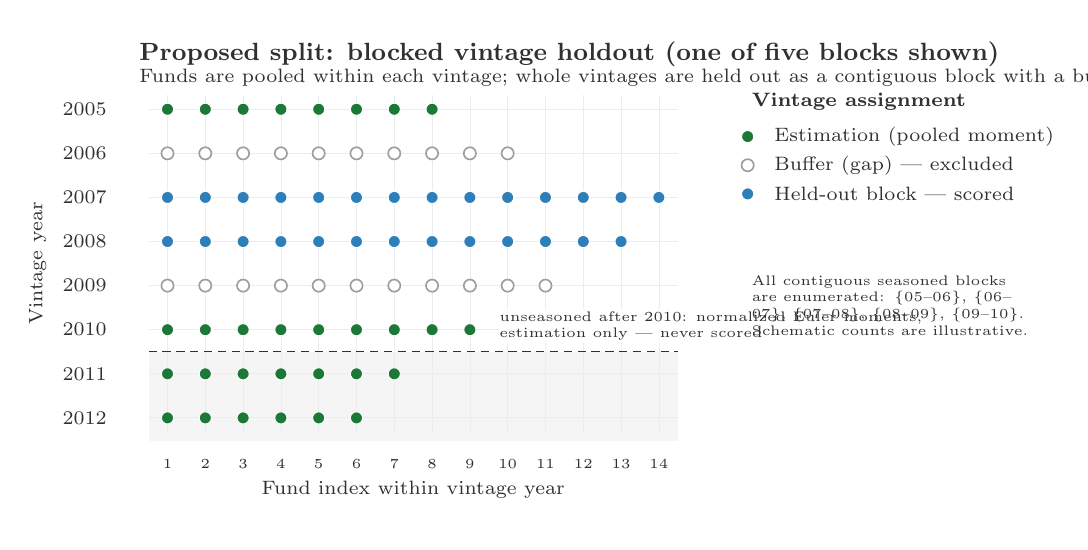
\begin{tikzpicture}[x=0.48cm,y=0.56cm]
	% Fixed white canvas so PDF-to-PNG conversion never creates a transparent margin.
	\path[use as bounding box] (-2.7,-9.35) rectangle (24.6,1.85);
	\fill[white] (-2.7,-9.35) rectangle (24.6,1.85);

	% Compact panel title. The paper caption should carry the full methodological text.
	\node[anchor=west, font=\bfseries\small, text=textgray] at (0,1.25)
		{Proposed split: blocked vintage holdout (one of five blocks shown)};
	\node[anchor=west, font=\scriptsize, text=textgray] at (0,0.72)
		{Funds are pooled within each vintage; whole vintages are held out as a contiguous block with a buffer.};

	% Light background for young vintages below the approach boundary.
	\fill[bandgray] (0.5,-5.5) rectangle (14.5,-7.52);

	% Grid and y-axis labels.
	\foreach \y/\year in {0/2005,-1/2006,-2/2007,-3/2008,-4/2009,-5/2010,-6/2011,-7/2012} {
		\draw[gridgray, line width=0.3pt] (0.5,\y) -- (14.5,\y);
		\node[anchor=east, font=\scriptsize, text=textgray] at (-0.35,\y) {\year};
	}

	% x-axis labels and faint vertical guides.
	\foreach \x in {1,...,14} {
		\draw[gridgray, line width=0.22pt] (\x,-7.32) -- (\x,0.32);
		\node[anchor=north, font=\tiny, text=textgray] at (\x,-7.72) {\x};
	}
	\node[anchor=north, font=\scriptsize, text=textgray] at (7.5,-8.2)
		{Fund index within vintage year};
	\node[rotate=90, anchor=south, font=\scriptsize, text=textgray] at (-1.95,-3.5)
		{Vintage year};

	% Vintage-level assignment: estimation / buffer / held-out block / unseasoned (estimation only).
	% 2005: estimation
	\foreach \x in {1,...,8} {\funddot{\x}{0}{estone}}
	% 2006: buffer (gap)
	\foreach \x in {1,...,10} {\gapdot{\x}{-1}}
	% 2007: held-out block
	\foreach \x in {1,...,14} {\funddot{\x}{-2}{validblue}}
	% 2008: held-out block
	\foreach \x in {1,...,13} {\funddot{\x}{-3}{validblue}}
	% 2009: buffer (gap)
	\foreach \x in {1,...,11} {\gapdot{\x}{-4}}
	% 2010: estimation
	\foreach \x in {1,...,9} {\funddot{\x}{-5}{estone}}
	% 2011: unseasoned, estimation only (Euler moments)
	\foreach \x in {1,...,7} {\funddot{\x}{-6}{estone}}
	% 2012: unseasoned, estimation only (Euler moments)
	\foreach \x in {1,...,6} {\funddot{\x}{-7}{estone}}

	% Approach-boundary annotation.
	\draw[densely dashed, textgray, line width=0.35pt] (0.5,-5.5) -- (14.5,-5.5);
	\node[anchor=west, align=left, font=\tiny, text=textgray, fill=white, fill opacity=0.9, text opacity=1, inner sep=1pt] at (9.7,-4.92)
		{unseasoned after 2010: normalized Euler moments,\\estimation only --- never scored};

	% Legend, placed to the right to avoid crowding the x-axis.
	\node[anchor=west, font=\bfseries\scriptsize, text=textgray] at (16.2,0.18)
		{Vintage assignment};
	\funddot{16.35}{-0.62}{estone}
	\node[anchor=west, font=\scriptsize, text=textgray] at (16.8,-0.62)
		{Estimation (pooled moment)};
	\gapdot{16.35}{-1.27}
	\node[anchor=west, font=\scriptsize, text=textgray] at (16.8,-1.27)
		{Buffer (gap) --- excluded};
	\funddot{16.35}{-1.92}{validblue}
	\node[anchor=west, font=\scriptsize, text=textgray] at (16.8,-1.92)
		{Held-out block --- scored};

	\node[anchor=west, align=left, text width=3.7cm, font=\tiny, text=textgray] at (16.2,-4.45)
		{All contiguous seasoned blocks are enumerated: \{05--06\}, \{06--07\}, \{07--08\}, \{08--09\}, \{09--10\}. Schematic counts are illustrative.};
\end{tikzpicture}
\end{document}
